\chapter{Metody algorytmiczne}\label{chap:algorithms}

W tym rozdziale przedstawiono wszystkie algorytmy zastosowane w pracy. Każdy algorytm opisano wraz z jego główną ideą, parametrami oraz analizą złożoności obliczeniowej.


Algorytmy zastosowane w pracy można podzielić na trzy grupy:
\begin{enumerate}
  \item \textbf{Metody dokładne} -- gwarantują znalezienie optymalnego rozwiązania: algorytm naiwny i programowanie całkowitoliczbowe (ILP).
  \item \textbf{Heurystyki konstrukcyjne} -- szybkie metody budujące rozwiązanie krok po kroku: algorytm zachłanny, zbiór dominujący, algorytm losowy.
  \item \textbf{Metaheurystyki} -- zaawansowane metody przeszukujące przestrzeń rozwiązań: algorytm genetyczny, przeszukiwanie tabu, algorytm mrówkowy, symulowane wyżarzanie.
\end{enumerate}

% \section{Formalizacja problemu}\label{sec:alg-conventions}

% Problem składa się z grafu $G=(V,E)$ oraz zbioru typów licencji $\mathcal{L}=\{\ell_1,\dots,\ell_T\}$. Każda licencja $\ell$ ma trzy parametry: koszt $c_\ell>0$, minimalną pojemność $l_\ell$ i maksymalną pojemność $u_\ell$, gdzie $1\le l_\ell\le u_\ell$.

% Grupa licencyjna składa się z właściciela $i$ (który kupuje licencję $\ell$) oraz członków grupy wybranych spośród sąsiadów właściciela. Oznaczając przez $N[i]$ zbiór składający się z wierzchołka $i$ i wszystkich jego sąsiadów, grupa licencyjna to podzbiór $G\subseteq N[i]$ taki, że właściciel $i$ należy do grupy ($i\in G$) oraz rozmiar grupy mieści się w dozwolonym zakresie ($l_\ell\le |G|\le u_\ell$).

% Rozwiązaniem problemu jest taki zbiór grup $\mathcal{S}$, że każdy wierzchołek grafu należy do dokładnie jednej grupy. Koszt rozwiązania to suma kosztów wszystkich utworzonych grup: $\cost(\mathcal{S})=\sum\limits_{(i,\ell,G)\in\mathcal{S}} c_\ell$.

\section{Metody dokładne}

\subsection{Algorytm naiwny}\label{subsec:naive}
Algorytm naiwny jest metodą dokładną. Działa dla wszystkich grafów. Przegląda wszystkie podziały zbioru wierzchołków na dopuszczalne grupy oraz wszystkie przypisania licencji. Wybierane jest rozwiązanie o najniższym koszcie. Liczba rozważanych konfiguracji rośnie nadwykładniczo, dlatego metoda ma znaczenie praktyczne tylko dla bardzo małych instancji.

Na rysunku \ref{fig:all_types_time} przedstawiono czasy obliczeń w funkcji liczby wierzchołków dla grafów losowych, małoświatowych i bezskalowych. Do 12 wierzchołków czas wykonania pozostaje akceptowalny dla celów eksperymentalnych. Powyżej tej wartości obserwuje się eksponencjalny wzrost złożoności czasowej, co czyni metodę niepraktyczną, zwłaszcza w kontekście dostępności bardziej efektywnych algorytmów, takich jak programowanie całkowitoliczbowe (ILP).

\begin{figure}[H]
  \centering
  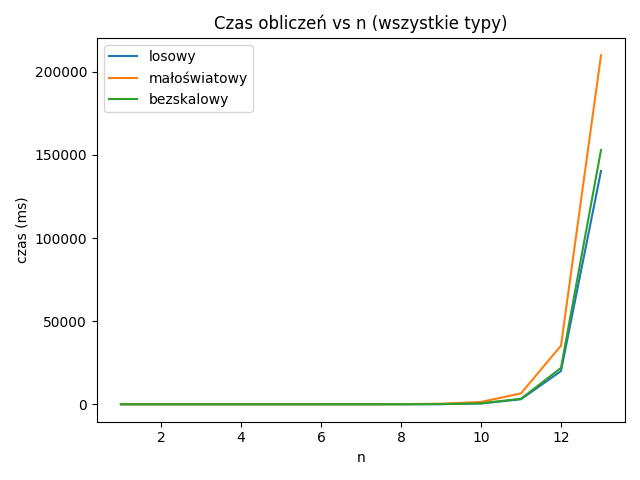
\includegraphics[width=0.66\textwidth]{assets/all_types_plot.png}
  \caption{Czas obliczeń algorytmu naiwnego w funkcji liczby wierzchołków n dla trzech typów grafów}
  \label{fig:all_types_time}
\end{figure}

\paragraph{Idea metody}
\begin{enumerate}
  \item Wygenerować wszystkie partycje zbioru \(V\).
  \item Dla każdego bloku partycji rozważyć wszystkich właścicieli oraz licencje spełniające ograniczenia pojemności.
  \item Odrzucić konfiguracje niespełniające warunków sąsiedztwa i pełnego pokrycia.
  \item Obliczyć koszt i zapamiętać najlepsze rozwiązanie.
\end{enumerate}

\begin{algorithm}[H]
  \caption{Algorytm naiwny: pełny przegląd rozwiązań}
  \label{alg:naive}
  \begin{algorithmic}[1]
    \Require graf \(G=(V,E)\), zbiory licencji \(\mathcal{L}\)
    \If{\(|V|>12\)} \State \Return przerwanie z powodu ograniczenia eksperymentalnego \EndIf
    \State \(best\_cost \gets \infty\), \(best \gets \emptyset\)
    \For{każda partycja \(P=\{P_1,\dots,P_k\}\) zbioru \(V\)}
    \For{każde przypisanie \(\ell\in\mathcal{L}\) i właściciela w każdym \(P_i\)}
    \If{spełnione pojemności, sąsiedztwo i pełne pokrycie}
    \State policz koszt; zaktualizuj \(best\), jeśli lepszy
    \EndIf
    \EndFor
    \EndFor
    \State \Return \(best\)
  \end{algorithmic}
\end{algorithm}

\paragraph{Złożoność}
Liczba partycji zbioru \(n\) elementów to liczba Bella \(B_n\). Zatem już sama enumeracja partycji kosztuje \(O(B_n)\). Dla każdej partycji rozważanych jest do \(O(n \cdot |\mathcal{L}|)\) wyborów właścicieli i licencji w blokach, z testami poprawności, co daje całkowity koszt rzędu \(O(B_n \cdot n \cdot |\mathcal{L}|)\).

Liczba Bella \(B_n\) to liczba wszystkich podziałów zbioru \(n\) elementów na niepuste, nierozróżnialne bloki. Równoważnie
\[
  B_n = \sum_{k=0}^{n} \left\{\!\!\begin{array}{c} n \\ k \end{array}\!\!\right\},
\]
gdzie symbole w nawiasach oznaczają liczby Stirlinga drugiego rodzaju. Liczby Bella spełniają także wzór Dobińskiego
\[
  B_n = \frac{1}{e}\sum_{k=0}^{\infty}\frac{k^{\,n}}{k!},
\]
oraz występują jako wartości wielomianów Toucharda w punkcie \(x=1\).

\subsection{Programowanie całkowitoliczbowe (ILP)}\label{subsec:ilp}

Programowanie całkowitoliczbowe formułuje problem jako zadanie minimalizacji kosztu z ograniczeniami liniowymi oraz binarnymi zmiennymi decyzyjnymi. Metoda jest dokładna i zwraca rozwiązanie optymalne, o ile solver zakończy się sukcesem.

\paragraph{Parametry i zmienne}
Niech \(\mathcal{L}\) będzie zbiorem typów licencji. Dla każdej licencji \(\ell\in\mathcal{L}\) dane są: koszt \(c_\ell>0\), minimalna pojemność \(l_\ell\ge 1\) oraz maksymalna pojemność \(u_\ell\ge l_\ell\). Dla każdego wierzchołka \(i\in V\) i licencji \(\ell\) definiowane są dwie rodziny binarnych zmiennych:
\begin{itemize}
  \item \(a_{i,\ell}\in\{0,1\}\) aktywacja grupy z właścicielem \(i\) i licencją \(\ell\) \((a_{i,\ell}=1\) gdy grupa istnieje\().\)
  \item \(x_{i,j,\ell}\in\{0,1\}\) przypisanie wierzchołka \(j\) do grupy właściciela \(i\) z licencją \(\ell\) \((x_{i,j,\ell}=1\) gdy \(j\) należy do tej grupy\().\)
\end{itemize}
Operowanie kosztami odbywa się przez \(c_\ell\). Ograniczenia pojemności wykorzystują \(l_\ell\) oraz \(u_\ell\).

\paragraph{Model matematyczny}
Dla \(N[i]=N(i)\cup\{i\}\) zapis modelu ma postać
\begin{align}
  \min\quad & \sum_{i\in V}\sum_{\ell\in\mathcal{L}} c_\ell\, a_{i,\ell}                    &  & \text{funkcja celu: suma kosztów aktywnych grup}                                    \\[4pt]
  \text{s.t.}\quad
            & \sum_{i\in N[j]}\sum_{\ell\in\mathcal{L}} x_{i,j,\ell} = 1                    &  & \forall j\in V \quad \text{pokrycie każdego wierzchołka dokładnie raz}              \\[2pt]
            & l_\ell\, a_{i,\ell} \le \sum_{j\in N[i]} x_{i,j,\ell} \le u_\ell\, a_{i,\ell} &  & \forall i\in V,\ \ell\in\mathcal{L} \quad \text{pojemność grupy zgodnie z licencją} \\[2pt]
            & x_{i,i,\ell} \ge a_{i,\ell}                                                   &  & \forall i\in V,\ \ell\in\mathcal{L} \quad \text{właściciel należy do własnej grupy} \\[2pt]
            & \sum_{\ell\in\mathcal{L}} a_{i,\ell} \le 1                                    &  & \forall i\in V \quad \text{co najwyżej jedna grupa na właściciela}                  \\[2pt]
            & a_{i,\ell}\in\{0,1\},\ x_{i,j,\ell}\in\{0,1\}                                 &  & \text{zmienne binarne.}
\end{align}


\paragraph{Interpretacja ograniczeń}
Pokrycie wymusza, aby każdy wierzchołek był przypisany do dokładnie jednej grupy. Pojemność wiąże rozmiar grupy z aktywacją i parametrami licencji: jeśli \(a_{i,\ell}=0\) to suma przypisań musi wynosić 0, a jeśli \(a_{i,\ell}=1\) to rozmiar zawiera się w \([l_\ell,u_\ell]\). Warunek właściciela gwarantuje obecność właściciela w swojej grupie. Ograniczenie jednej grupy na właściciela zapobiega tworzeniu wielu grup startujących w tym samym węźle. Zerowanie \(x_{i,j,\ell}\) poza \(N[i]\) formalizuje wymóg, że członkowie grupy są właścicielem lub jego sąsiadami.

\paragraph{Złożoność i zastosowanie}
Rozmiar modelu jest rzędu \(O(|V|\cdot|\mathcal{L}|\cdot \Delta)\) zmiennych, gdzie \(\Delta\) oznacza maksymalny stopień grafu. W gęstych sieciach rośnie liczba zmiennych i ograniczeń, co może wydłużać czas rozwiązania. W pracy ILP służy jako punkt odniesienia jakości, jako metoda do małych i średnich instancji oraz jako źródło górnych ograniczeń dla metaheurystyk.

\paragraph{Implementacja}
Model zaimplementowano w Pythonie z użyciem biblioteki \texttt{PuLP}. Jako solver zastosowano \texttt{CBC} przez klasę \texttt{pulp.PULP\_CBC\_CMD}. Zmienne \(\{0,1\}\) są interpretowane progowo przy rekonstrukcji rozwiązania \((>0.5\) traktowane jako prawda\().\) Strukturę zmiennych odpowiadających \(a_{i,\ell}\) i \(x_{i,j,\ell}\), funkcję celu oraz powyższe ograniczenia odwzorowano bezpośrednio, zgodnie z kodem solvera używanym w eksperymentach.

\section{Heurystyki konstrukcyjne}

\subsection{Algorytm zachłanny}\label{subsec:greedy}

Algorytm zachłanny to szybka heurystyka, która buduje rozwiązanie krok po kroku, w każdym kroku wybierając lokalnie najlepszą opcję. Algorytm nie gwarantuje znalezienia optymalnego rozwiązania, ale jest bardzo szybki i daje zazwyczaj w miarę dobre wyniki.

\paragraph{Idea metody}
Algorytm działa według następującej strategii:
\begin{enumerate}
  \item Sortuje wierzchołki nierosnąco według liczby sąsiadów (stopnia wierzchołka).
  \item Dla każdego wierzchołka sprawdza, czy może być właścicielem grupy.
  \item Wybiera typ licencji i rozmiar grupy tak, aby zminimalizować stosunek kosztu do rozmiaru grupy.
  \item Dodaje członków do grupy wybierając wierzchołki o największej liczbie sąsiadów.
  \item Powtarza proces dla wszystkich niepokrytych wierzchołków.
\end{enumerate}

Algorytm nie ma parametrów do dostrajania. Wszystkie decyzje są podejmowane deterministycznie na podstawie struktury grafu i kosztów licencji, choć w przypadku wierzchołków o tym samym stopniu kolejność wyboru może wpływać na wynik końcowy.

Sortowanie według stopnia wierzchołka (liczby sąsiadów) sprawdza się dobrze w praktyce, ponieważ wierzchołki o wysokim stopniu mogą tworzyć większe, bardziej efektywne grupy licencyjne.

\begin{algorithm}[H]
  \caption{Algorytm zachłanny}
  \label{alg:greedy}
  \begin{algorithmic}[1]
    \Require graf $G=(V,E)$, typy licencji $\mathcal{L}$
    \State posortuj wierzchołki nierosnąco według stopnia
    \State $niepokryte \gets V$
    \For{każdy wierzchołek $v$ w posortowanej kolejności}
    \If{$v$ już pokryty} \textbf{continue} \EndIf
    \State znajdź dostępnych sąsiadów $v$ wśród niepokrytych
    \For{każdy typ licencji $\ell$}
    \State oblicz efektywność: $koszt_\ell / rozmiar\_grupy$
    \EndFor
    \State wybierz licencję i członków grupy o najlepszej efektywności
    \State utwórz grupę z $v$ jako właścicielem
    \State usuń członków grupy z $niepokryte$
    \EndFor
    \State \Return utworzone grupy
  \end{algorithmic}
\end{algorithm}


\paragraph{Złożoność i zastosowanie}
Algorytm ma złożoność czasową $O(nT + m\log n)$, gdzie $n$ to liczba wierzchołków, $T$ to liczba typów licencji, a $m$ to liczba krawędzi.
Algorytm zachłanny jest bardzo szybki i daje stabilne wyniki. Z tego powodu często używany był jako:
\begin{itemize}
  \item podstawowa metoda do porównywania z innymi algorytmami,
  \item źródło rozwiązania początkowego dla bardziej zaawansowanych metod,
  \item szybka metoda dla dużych grafów, gdzie inne algorytmy są zbyt wolne.
\end{itemize}
Wadą algorytmu jest to, że podejmując lokalnie najlepsze decyzje, może przegapić lepsze rozwiązania globalne.
\subsection{Heurystyka zbioru dominującego}\label{subsec:ds}

Heurystyka korzysta z konstrukcji \emph{minimalnych względem inkluzji} zbiorów dominujących. Zbiór dominujący jest minimalny, gdy usunięcie dowolnego jego wierzchołka powoduje utratę własności dominowania \cite{haynes1998domination}. W kontekście licencjonowania dominatorem nazywa się wierzchołek wybrany do zbioru dominującego, który stanie się właścicielem grupy licencyjnej i pokryje siebie oraz swoich sąsiadów.

Wskaźnik wyboru kandydata opiera się na \(\mathrm{coverage}(v)\) oraz \(\min\_\mathrm{cpn}(v)\).
\begin{itemize}
  \item \(\mathrm{coverage}(v)=|(N(v)\cup\{v\})\cap U|\) to liczba jeszcze niepokrytych węzłów, które może pokryć \(v\).
  \item \(\min\_\mathrm{cpn}(v)\) to minimalny koszt na węzeł dla \(v\), liczony po wszystkich licencjach i dopuszczalnych rozmiarach grupy:
        \[
          \min\_\mathrm{cpn}(v)=\min_{\ell\in\mathcal{L}}\;\min_{s\in[l_\ell,\;\min\{u_\ell,\ \mathrm{coverage}(v)\}]}\ \frac{c_\ell}{s}.
        \]
        Interpretacja: wybieramy dla \(v\) najkorzystniejszą licencję i rozmiar grupy, które dają najniższy koszt jednostkowy.
\end{itemize}

\begin{algorithm}[H]
  \caption{Zbiór dominujący z budowaniem grup}\label{alg:ds}
  \begin{algorithmic}[1]
    \Require graf $G=(V,E)$, zbiory licencji $\mathcal{L}$
    \State $U\gets V$, $D\gets\emptyset$
    \While{$U\neq\emptyset$}
    \State dla każdego $v\in V$ policz $\mathrm{coverage}(v)=|(N(v)\cup\{v\})\cap U|$ oraz $\min\_\mathrm{cpn}(v)$
    \State wybierz $u$ maksymalizujące $\mathrm{coverage}(v)/\min\_\mathrm{cpn}(v)$; jeśli brak rozstrzygnięcia wybierz dowolne $u\in U$
    \State $D\gets D\cup\{u\}$, $U\gets U\setminus(N(u)\cup\{u\})$
    \EndWhile
    \State posortuj $D$ nierosnąco po $\deg$
    \For{każde $u\in D$ oraz dla pozostałych nieprzydzielonych węzłów}
    \State $S\gets (N(u)\cup\{u\})\cap$ nieprzydzieleni
    \State wybierz najtańszą dopuszczalną licencję dla $u$ i zbuduj największą dopuszczalną grupę w $S$; w ostateczności przydziel licencję indywidualną
    \EndFor
    \State \Return utworzone grupy
  \end{algorithmic}
\end{algorithm}

\paragraph{Złożoność i zastosowanie}
Faza wyboru dominatorów w każdej rundzie przechodzi po wszystkich wierzchołkach, ich sąsiadach i typach licencji, co daje koszt rzędu \(O(n m T)\). Faza budowania grup dla każdego dominatora sortuje kandydatów i sprawdza warianty licencji. W gęstych grafach rośnie to do \(O(n^3 T \log n)\), w rzadkich pozostaje bliżej \(O(n m T)\). Heurystyka szybko daje kompletne pokrycie i stanowi dobre rozwiązanie startowe dla metod ulepszających.

\subsection{Algorytm losowy}\label{subsec:random}

Algorytm losowy pełni rolę metody odniesienia do oceny jakości rozwiązań generowanych przez inne algorytmy. Weryfikuje poprawność implementacji i stanowi stochastyczny punkt odniesienia. Wierzchołki są przetwarzane w losowej kolejności, a wybór licencji i składu grupy jest losowy w granicach ograniczeń pojemności i sąsiedztwa.

\paragraph{Idea metody}
\begin{enumerate}
  \item Losowana jest kolejność przetwarzania wierzchołków.
  \item Dla bieżącego wierzchołka wyznaczany jest zbiór kandydatów obejmujący jego oraz nieprzydzielonych sąsiadów.
  \item Jeżeli istnieje dopuszczalna licencja, losowany jest typ licencji, rozmiar grupy oraz członkowie grupy z dostępnych kandydatów.
        Rozważano wariant wyboru zgodnie z najlepszym kosztem jednostkowym \(\min_{\ell,s} c_\ell/s\), analogicznie do heurystyki dominującej.
        W tej pracy przyjęto jednak minimalną deterministyczność i maksymalną losowość do wyznaczenia górnej granicy efektywności metaheurystyk.
  \item W przeciwnym razie przydzielana jest najtańsza dostępna licencja indywidualna.
  \item Kroki są powtarzane do pełnego pokrycia grafu.
\end{enumerate}

\paragraph{Uwagi o losowości}
Celem było uzyskanie szerokiego spektrum wyników, które odzwierciedla czysty przypadek pod ograniczeniami problemu.
Wariant z wyborem licencji według najlepszego kosztu na węzeł wprowadzałby element kierowany, który spłaszczałby rozkład wyników.
Testowano koncepcję wielu restartów, na przykład stu uruchomień z wyborem najlepszego wyniku.
Ze względu na dużą wariancję przypisań i wysoką losowość na etapie doboru licencji i składu grup obserwowane korzyści z wielokrotnych restartów były niewielkie względem średniej jednego przebiegu.
Z tego powodu stosowany jest pojedynczy przebieg z opcjonalnym nasionem generatora liczb losowych, co pozwala odtwarzać eksperymenty.

\begin{algorithm}[H]
  \caption{Losowy dobór licencji i składu grupy}\label{alg:randomized}
  \begin{algorithmic}[1]
    \Require graf $G=(V,E)$, zbiory licencji $\mathcal{L}$
    \State $U\gets V$, $\pi\gets$ losowa permutacja $V$
    \For{node w kolejności $\pi$}
    \If{$node\notin U$} \textbf{continue} \EndIf
    \State $S\gets \bigl(N(node)\cup\{node\}\bigr)\cap U$
    \If{istnieje licencja $\ell$ z $l_\ell\le |S|$}
    \State losuj $\ell$ oraz rozmiar $s\in\bigl[l_\ell,\min\{|S|,u_\ell\}\bigr]$, następnie losuj członków grupy z $S$
    \Comment{wariant kierowany: można zastąpić wyborem $\arg\min_{\ell,s} c_\ell/s$}
    \Else
    \State przydziel najtańszą licencję indywidualną
    \EndIf
    \State dodaj grupę, usuń jej członków z $U$
    \EndFor
    \While{$U\neq\emptyset$} przydziel najtańszą licencję indywidualną i usuń węzeł z $U$ \EndWhile
  \end{algorithmic}
\end{algorithm}

\paragraph{Złożoność i zastosowanie}
Każdy wierzchołek i jego sąsiedzi są przeglądani co najwyżej raz, a przy każdej próbie losowania licencji przeglądane są wszystkie typy licencji, co daje koszt rzędu \(O\bigl(T(m+n)\bigr)\).
W gęstych grafach upraszcza się to do \(O(Tn^2)\).
Algorytm służy jako benchmark stochastyczny oraz kontrola jakości innych metod.
Wariant kierowany \(\min c_\ell/s\) nie zmienia rzędu złożoności i może być użyty pomocniczo do analizy wrażliwości.


\section{Metaheurystyki}

Metaheurystyki to zaawansowane algorytmy przeszukujące przestrzeń rozwiązań w sposób inteligentny. W przeciwieństwie do heurystyk konstrukcyjnych, które budują rozwiązanie od zera, metaheurystyki zaczynają od pewnego rozwiązania i systematycznie je poprawiają.

\paragraph{Dobór parametrów}
Parametry metaheurystyk zostały dobrane eksperymentalnie na podstawie testów na grafach różnych rozmiarów.

\paragraph{Operacje modyfikacji rozwiązania}
Metaheurystyki poprawiają rozwiązanie stosując następujące operacje:
\begin{itemize}
  \item zmiana typu licencji używanej przez właściciela grupy
  \item przeniesienie członka z jednej grupy do drugiej
  \item zamiana miejscami dwóch członków z różnych grup
  \item scalanie dwóch grup w jedną lub rozdzielanie na dwie dopuszczalne.
\end{itemize}

\subsection{Algorytm genetyczny}\label{subsec:ga}
Algorytm genetyczny utrzymuje populację pełnych przydziałów licencyjnych i z pokolenia na pokolenie ulepsza je, korzystając z losowych mutacji i krzyżowania par rodziców \cite{holland1975,goldberg1989}. Zaczyna od kilku rozwiązań zachłannych i losowych, a następnie w każdej generacji wybiera najlepsze osobniki (elita), losuje rodziców metodą turniejową i tworzy potomstwo przez krzyżowanie lub mutację. Słabsze rozwiązania są stopniowo zastępowane lepszymi, a algorytm zapamiętuje najlepszy znaleziony koszt.

\paragraph{Parametry}
\begin{itemize}
  \item \textbf{Wielkość populacji} $P=30$ - liczba rozwiązań utrzymywanych w każdej generacji.
  \item \textbf{Liczba pokoleń} $G=40$ - maksymalna liczba iteracji ewolucji.
  \item \textbf{Udział elity} $\alpha=20\%$ - część najlepszych osobników kopiowana bez zmian do kolejnego pokolenia.
  \item \textbf{Prawdopodobieństwo krzyżowania} $p_c=60\%$ - przy tej szansie dziecko powstaje przez połączenie dwóch rodziców; w przeciwnym razie wykonywana jest mutacja.
\end{itemize}

\begin{algorithm}[H]
  \caption{Algorytm genetyczny}
  \label{alg:ga}
  \begin{algorithmic}[1]
    \Require graf $G=(V,E)$, typy licencji $\mathcal{L}$
    \State utwórz populację początkową (zachłanny + losowe rozwiązania)
    \For{każde pokolenie}
    \State oceń wszystkie rozwiązania (funkcja kosztu)
    \State zachowaj elitę (najlepsze rozwiązania)
    \While{populacja niepełna}
    \If{losowanie krzyżowania}
    \State wybierz dwóch rodziców (selekcja turniejowa)
    \State skrzyżuj rodziców (połącz efektywne grupy)
    \Else
    \State wybierz rozwiązanie i zmutuj (operacje sąsiedztwa)
    \EndIf
    \State dodaj potomka do nowej populacji
    \EndWhile
    \State zaktualizuj najlepsze znalezione rozwiązanie
    \EndFor
    \State \Return najlepsze rozwiązanie
  \end{algorithmic}
\end{algorithm}

\paragraph{Złożoność i zastosowanie}
Inicjalizacja populacji korzysta z jednego osobnika otrzymanego za pomocą algorytmu zachłannego i $P-1$ losowych rozwiązań, co kosztuje około $O\bigl(P \cdot (nT + m\log n)\bigr)$. Każda generacja sortuje populację ($O(P\log P)$), a następnie tworzy nowe pokolenie. Mutacje wywołują ograniczoną liczbę operatorów sąsiedztwa (zmiana typu licencji, przeniesienie członka, zamiana miejscami, scalanie lub podział grup), a krzyżowanie w razie potrzeby uruchamia heurystykę zachłanną na podgrafie, co razem daje koszt rzędu $O(nT + m\log n)$ na potomka. Łącznie otrzymujemy $O\bigl(G \cdot P \cdot (nT + m\log n)\bigr)$ w najgorszym przypadku. Algorytm działa wolniej od prostych heurystyk, ale potrafi znacząco poprawić ich wyniki i służy jako główna metoda poszukiwania wysokiej jakości rozwiązań, gdy możemy poświęcić na optymalizację więcej czasu.


\subsection{Przeszukiwanie tabu}\label{subsec:tabu}
Algorytm tabu rozpoczyna działanie od rozwiązania uzyskanego heurystyką zachłanną, a następnie iteracyjnie przeszukuje lokalne sąsiedztwo. Sąsiadem nazywa się rozwiązanie otrzymane przez pojedynczą operację mutacji, na przykład zmianę typu licencji właściciela, przeniesienie członka między grupami, zamianę członków lub scalenie i podział grup. Lista tabu przechowuje podpisy ostatnich rozwiązań lub ruchów i zakazuje wyboru kandydatów, którzy prowadzą do niedawno odwiedzonych stanów. Kryterium aspiracji pozwala pominąć zakaz, gdy kandydat poprawia najlepszy dotąd koszt. Mechanizm ten ogranicza krótkie cykle i równoważy lokalne doskonalenie z eksploracją nowych przydziałów licencji \cite{glover1989}.

\paragraph{Parametry}
\begin{itemize}
  \item \textbf{Maksymalna liczba iteracji} \(I=1000\).
  \item \textbf{Długość listy tabu} \(L=20\) elementów.
  \item \textbf{Liczba sąsiadów na iterację} \(k=10\).
\end{itemize}

\begin{algorithm}[H]
  \caption{Przeszukiwanie tabu}\label{alg:tabu}
  \begin{algorithmic}[1]
    \Require graf \(G=(V,E)\), typy licencji \(\mathcal{L}\)
    \State \(aktualne \gets\) rozwiązanie początkowe wyznaczone algorytmem zachłannym
    \State \(najlepsze \gets aktualne\)
    \State \(lista\_tabu \gets\) pusta kolejka o stałej długości \(L\); wstaw podpis \(aktualne\)
    \For{każdą iterację}
    \State wygeneruj sąsiedztwo \(aktualne\) przez operacje mutacji
    \State wybierz najlepszego kandydata, którego podpis nie znajduje się na \(lista\_tabu\) lub który poprawia \(najlepsze\) \((\)aspiracja\()\)
    \If{wybrano kandydata}
    \State \(aktualne \gets\) kandydat; zaktualizuj \(lista\_tabu\)
    \If{\(aktualne\) lepsze niż \(najlepsze\)} \State \(najlepsze \gets aktualne\) \EndIf
    \Else
    \State \textbf{przerwij}
    \EndIf
    \EndFor
    \State \Return \(najlepsze\)
  \end{algorithmic}
\end{algorithm}

Pojemność oznacza ograniczenia licencji na rozmiar grupy, to jest przedział \([l_\ell,u_\ell]\). Pokrycie oznacza warunek, że każdy wierzchołek należy do dokładnie jednej grupy. Sąsiedztwo oznacza zbiór rozwiązań osiągalnych z bieżącego przez pojedynczą operację mutacji.

\paragraph{Złożoność i zastosowanie}
Inicjalizacja obejmuje jedno uruchomienie heurystyki zachłannej \(O(nT + m\log n)\). W każdej z \(I\) iteracji generowanych jest do \(k\) sąsiadów. Ocena kandydata obejmuje sprawdzenie pojemności, pokrycia i zgodności z sąsiedztwem w grafie, co kosztuje około \(O(nT + m)\). Łączna złożoność wynosi w przybliżeniu \(O\!\left(I \cdot k \cdot (nT + m)\right)\). Przeszukiwanie tabu dobrze sprawdza się jako metoda ulepszająca: poprawia rozwiązania wyjściowe przy umiarkowanym czasie obliczeń i ogranicza powroty do niedawno odwiedzonych stanów dzięki liście tabu.

\subsection{Algorytm mrówkowy}\label{subsec:aco}
Algorytm mrówkowy buduje wiele rozwiązań równolegle. Każda mrówka konstruuje przydział licencji, kierując się siłą śladów feromonowych (informacja o dotychczas dobrych wyborach) oraz heurystyką preferującą wierzchołki o dużym stopniu i licencje o dobrym stosunku pojemności do ceny \cite{dorigo1997}. Po każdej iteracji feromony parują, a najlepsze dotąd rozwiązanie wzmacnia ścieżki, dzięki czemu kolejne mrówki chętniej eksplorują obiecujące fragmenty przestrzeni.

\paragraph{Parametry}
\begin{itemize}
  \item \textbf{Waga feromonu} $\alpha=1,0$ -- określa, jak mocno mrówki ufają dotychczasowym śladom.
  \item \textbf{Waga heurystyki} $\beta=2,0$ -- wzmacnia preferencję dla lokalnie dobrych decyzji (wysoki stopień, tanie licencje).
  \item \textbf{Tempo parowania} $\rho=0,5$ -- część feromonu usuwana po każdej iteracji.
  \item \textbf{Prawdopodobieństwo wyboru zachłannego} $q_0=0,9$ -- z tą szansą mrówka wybiera najlepszą dostępnie opcję, w przeciwnym razie losuje proporcjonalnie do wag.
  \item \textbf{Liczba mrówek} $A=20$ -- ile rozwiązań konstruujemy równolegle w jednej iteracji.
  \item \textbf{Maksymalna liczba iteracji} $I=100$ -- ile razy aktualizujemy feromony.
  \item \textbf{Losowe nasiono} (opcjonalne) -- pozwala odtworzyć przebieg eksperymentu.
\end{itemize}


\begin{algorithm}[H]
  \caption{Algorytm mrówkowy}
  \label{alg:aco}
  \begin{algorithmic}[1]
    \Require graf $G=(V,E)$, typy licencji $\mathcal{L}$
    \State zainicjalizuj feromony $\tau$ (dla par wierzchołek-licencja)
    \State zainicjalizuj heurystyki $\eta$ (na podstawie stopni wierzchołków i kosztów licencji)
    \State $najlepsze \gets$ rozwiązanie początkowe (zachłanne)
    \For{każdą iterację}
    \For{każdą mrówkę}
    \State $niepokryte \gets V$
    \While{$niepokryte \neq \emptyset$}
    \State wybierz właściciela na podstawie $\tau$ i $\eta$ (reguła wyboru lub ruletka)
    \State wybierz typ licencji na podstawie $\tau$ i $\eta$
    \State utwórz grupę, usuń członków z $niepokryte$
    \EndWhile
    \If{mrówka znalazła lepsze rozwiązanie}
    \State $najlepsze \gets$ rozwiązanie mrówki
    \EndIf
    \EndFor
    \State wyparuj część feromonów: $\tau \gets \tau \cdot (1-evaporation)$
    \State wzmocnij feromony na ścieżce $najlepsze$: $\tau \gets \tau + 1/koszt$
    \EndFor
    \State \Return $najlepsze$
  \end{algorithmic}
\end{algorithm}

\paragraph{Złożoność i zastosowanie}
Inicjalizacja feromonów i heurystyk kosztuje $O(nT)$. Pojedyncza konstrukcja rozwiązania wymaga odwiedzenia przez mrówkę każdego wierzchołka co najwyżej raz. Przy wyborze właściciela w każdej decyzji oceniani są wszyscy kandydaci i wszystkie licencje. Prowadzi to do złożoności czasowej około $O(n^2 T + m\log n)$ na jedną mrówkę, z uwzględnieniem sortowania sąsiadów. Algorytm wykonujący $I$ iteracji z $A$ mrówkami ma więc złożoność rzędu $O\!\left(I \cdot A \cdot (n^2 T + m\log n)\right)$. Metoda jest bardziej złożona obliczeniowo niż tabu i algorytm zachłanny, ale pozwala eksplorować wiele alternatywnych konfiguracji i stopniowo wzmacniać najlepsze z nich.


\subsection{Symulowane wyżarzanie }\label{subsec:sa}
Symulowane wyżarzanie rozpoczyna od rozwiązania zachłannego i w każdej iteracji losuje ruch sąsiedztwa (zmiana licencji, przeniesienie członka, zamiana, scalenie lub podział grupy). Nowy stan jest akceptowany zawsze, gdy obniża koszt, a czasami także wtedy, gdy go pogarsza - z prawdopodobieństwem zależnym od bieżącej temperatury \(T\) i różnicy kosztów \cite{kirkpatrick1983}. Temperatura maleje według ustalonego współczynnika, a gdy algorytm zbyt długo nie znajduje poprawy, dodatkowo jest obniżana o połowę. Dzięki temu metoda potrafi opuszczać lokalne minima i stopniowo stabilizuje się w pobliżu dobrego rozwiązania.

\paragraph{Parametry}
\begin{itemize}
  \item \textbf{Temperatura początkowa} $T_0 = 100.0$ - początkowy poziom losowości przy akceptacji gorszych ruchów.
  \item \textbf{Współczynnik chłodzenia} $\alpha = 0.995$ - w każdej iteracji temperatura jest mnożona przez $\alpha$.
  \item \textbf{Temperatura minimalna} $T_{\min} = 0.001$ - po jej osiągnięciu algorytm kończy działanie.
  \item \textbf{Maksymalna liczba iteracji} $I = 20\,000$ - górne ograniczenie liczby kroków.
  \item \textbf{Limit stagnacji} $S = 2\,000$ - po tylu nieudanych próbach temperatura jest dodatkowo dzielona przez 2.
\end{itemize}

\begin{algorithm}[H]
  \caption{Symulowane wyżarzanie}
  \label{alg:sa}
  \begin{algorithmic}[1]
    \Require graf $G=(V,E)$, typy licencji $\mathcal{L}$
    \State $aktualne \gets$ rozwiązanie początkowe (zachłanne)
    \State $najlepsze \gets aktualne$
    \State $temperatura \gets T_0$ (początkowa temperatura)
    \For{każdą iterację}
    \If{$temperatura < T_{min}$} \textbf{break} \EndIf
    \State wybierz losową operację sąsiedztwa
    \State $kandydat \gets$ wynik operacji sąsiedztwa
    \State $\Delta \gets koszt(kandydat) - koszt(aktualne)$
    \If{$\Delta \leq 0$ LUB $random() < \exp(-\Delta / temperatura)$}
    \State $aktualne \gets kandydat$
    \If{$koszt(kandydat) < koszt(najlepsze)$}
    \State $najlepsze \gets kandydat$
    \EndIf
    \EndIf
    \State $temperatura \gets temperatura \cdot cooling\_rate$
    \EndFor
    \State \Return $najlepsze$
  \end{algorithmic}
\end{algorithm}

\paragraph{Złożoność i zastosowanie}
Inicjalizacja wymaga jednego wywołania heurystyki zachłannej działającej w czasie $O(nT + m\log n)$. Każda iteracja wykonuje ograniczoną liczbę prób wygenerowania sąsiada (do 12 ruchów), a zaakceptowany kandydat przechodzi pełną walidację pokrycia i ograniczeń, co ma złożoność około $O(nT + m)$. W rezultacie złożoność obliczeniowa całego przebiegu wynosi $O\bigl(I \cdot (nT + m)\bigr)$ z dodatkowym mnożnikiem wynikającym z limitu stagnacji. Symulowane wyżarzanie jest umiarkowanie złożone obliczeniowo, ale często zapewnia lepsze rozwiązania niż czyste metody lokalne, szczególnie gdy potrzebna jest możliwość wychodzenia z lokalnych minimów przy ograniczonym czasie działania.
